\section{Nivel III: ecualizador de fase pasatodo}
\label{sec:nivel3}

Un filtro Chebyshev transmite la banda de paso con poca variación de amplitud, pero no con retardo constante. Su retardo de grupo crece hacia el
borde de la banda (\cref{sec:mediciones}), de modo que las componentes de una señal cercanas a \qty{1}{\kilo\hertz} llegan más tarde que las de baja
frecuencia y la forma de onda se deforma (sobrepico y oscilación en la respuesta al escalón). Este nivel optativo diseña, simula, construye y mide un
ecualizador pasatodo que compensa esa variación \emph{en el prototipo construido}. El procesamiento está en el notebook~06.

\subsection{Banda útil y función objetivo}
\paragraph{Filtro a ecualizar.} El ecualizador se diseña para el prototipo, no para el filtro nominal, con el modelo ajustado a la medición del
filtro (\cref{sec:mediciones}: $f_r = \qr{1}{\eProtoFr}{\hertz}$, $f_0 = \qr{1}{\eProtoFo}{\hertz}$, $Q = \nr{3}{\eProtoQ}$). Su retardo de grupo, calculado
polo a polo, vale \qty{\eTauCeroF}{\milli\second} en baja frecuencia y \qty{\eTauUnokF}{\milli\second} en \qty{1}{\kilo\hertz}, con un máximo cerca
de \qty{1.15}{\kilo\hertz} (\cref{fig:ec_objetivo}). La distinción importa: el ecualizador óptimo para el prototipo, aplicado al filtro nominal, solo
reduce la variación de \qty{\eJNomSinEc}{\milli\second} a \qty{\eJNomConEcProto}{\milli\second}, porque los dos filtros difieren en unos pocos por
ciento en $f_r$ y $f_0$.

\paragraph{Banda útil.} Es la banda de paso de la plantilla, $0 < f \le f_p = \qty{1}{\kilo\hertz}$: la que el filtro transmite y en la que importa
la forma de onda. Por encima de $f_p$ la señal está atenuada y su retardo no tiene consecuencias.

\paragraph{Función objetivo.} Un retardo constante solo desplaza la señal en el tiempo; lo que la deforma es la \emph{variación} del retardo. Se
minimiza entonces la variación pico a pico del retardo total en la banda útil (criterio \emph{minimax}),
\begin{equation}
  J = \max_{0 < f \le f_p} \tau_\text{tot}(f) - \min_{0 < f \le f_p} \tau_\text{tot}(f), \qquad \tau_\text{tot} = \tau_\text{filtro} + \tau_\text{ec},
  \label{eq:J_ecualizador}
\end{equation}
y como medida complementaria se informa el valor eficaz de la desviación respecto de la media, $J_\text{rms}$. Sin ecualizar,
$J = \qr{3}{\eJsinEc}{\milli\second}$ (\qty{50}{\percent} del retardo en continua). El precio de ecualizar es un retardo total mayor, que para la mayoría
de las aplicaciones (audio, instrumentación) no tiene consecuencias.

\begin{figure}[H]
  \centering
  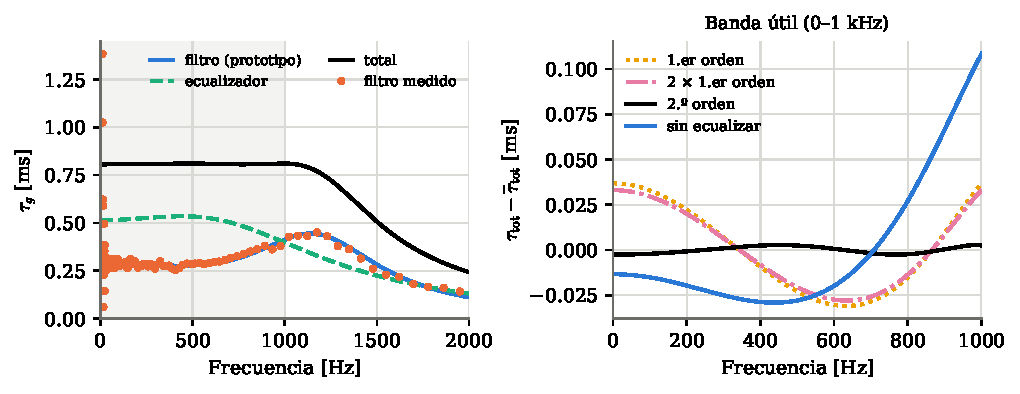
\includegraphics[width=\textwidth]{fig_ec_objetivo}
  \caption{Izquierda: retardo de grupo del prototipo (modelo ajustado y medición), del ecualizador de 2.º orden óptimo y de la cascada. Derecha:
  desviación del retardo total respecto de su media en la banda útil, para las alternativas de la \cref{tab:ec_orden}.}
  \label{fig:ec_objetivo}
\end{figure}

\subsection{Orden del ecualizador}
Para aplanar $\tau_\text{tot}$, el ecualizador debe aportar mucho retardo en baja frecuencia y poco cerca de $f_p$. Se compararon cuatro
alternativas, optimizando $J$ en cada caso (\cref{tab:ec_orden}). Los pasatodos de 1.er orden, cuyo retardo $2\omega_a/(\omega_a^2+\omega^2)$
decrece demasiado despacio, apenas reducen $J$ a la mitad, incluso con dos secciones. El pasatodo de 2.º orden
\begin{equation}
  H_\text{ec}(s) = k\,\frac{s^2 - (\omega_0/Q)\,s + \omega_0^2}{s^2 + (\omega_0/Q)\,s + \omega_0^2}
\end{equation}
tiene un retardo casi plano hasta unos \qty{600}{\hertz} que cae justo donde sube el del filtro: con $f_0 = \qty{\eFoAP}{\hertz}$ y
$Q = \num{\eQAP}$ reduce $J$ a \qty{\eJOpt}{\milli\second}, \num{\eMejoraOpt} veces menos, con un solo AO. Agregarle una sección de 1.er orden
mejora el óptimo teórico (\qty{\eJDosMasUno}{\milli\second}), pero esa mejora no es alcanzable: como se muestra más adelante, con componentes reales
$J$ queda limitado por la dispersión de $f_0$ y $Q$ del ecualizador mucho antes de llegar al óptimo de un solo AO. Se elige entonces el pasatodo
de 2.º orden con un AO.

\begin{table}[H]
  \centering\small
  \caption{Alternativas de ecualizador para el prototipo, con sus parámetros óptimos. La mejora es el cociente entre $J$ sin ecualizar y $J$ con el
  ecualizador; $\tau_\text{tot}(0)$ es el retardo total en continua.}
  \label{tab:ec_orden}
  \tabres{tab_ec_orden}
\end{table}

\subsection{Topología y derivación}
Se usa una celda de un solo AO (\cref{fig:ec_esquema}): un pasabanda de realimentación múltiple (Delyiannis--Friend) que recibe la entrada a través
de $R_1$ y una fracción $k = R_b/(R_a+R_b)$ de la misma entrada en la entrada no inversora. El análisis nodal con AO ideal ($V_- = V_+ = kV_e$),
hecho con SymPy antes de imponer valores, da
\begin{equation}
  H_\text{ec}(s) = \frac{k\left[s^2 + b_1 s + \omega_0^2\right]}{s^2 + \dfrac{C_1+C_2}{R_2C_1C_2}\,s + \dfrac{1}{R_1R_2C_1C_2}}, \qquad
  b_1 = \frac{k(C_1R_1 + C_1R_2 + C_2R_1) - C_1R_2}{k\,C_1C_2R_1R_2},
\end{equation}
con $\omega_0 = 1/\sqrt{R_1R_2C_1C_2}$ y $Q = \sqrt{R_2/R_1}\,\sqrt{C_1C_2}/(C_1+C_2)$.

\begin{figure}[H]
  \centering
  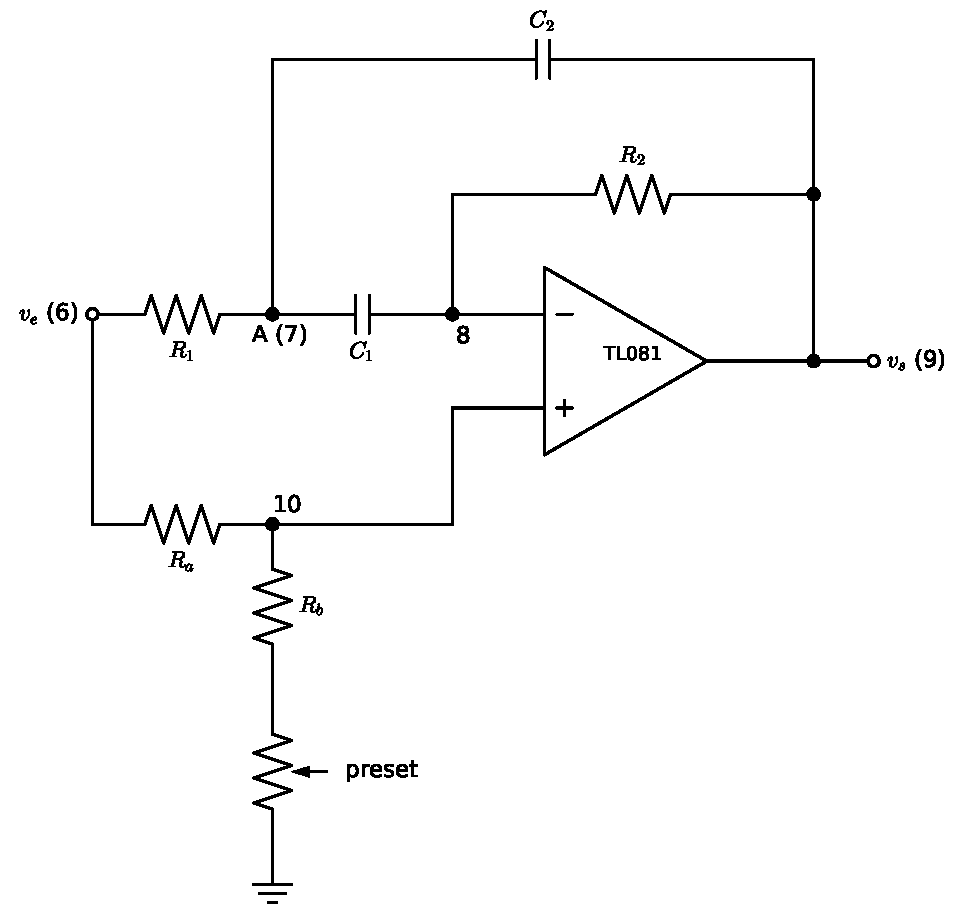
\includegraphics[width=0.62\textwidth]{fig_ec_esquema}
  \caption{Ecualizador pasatodo de 2.º orden con un AO (TL081). El preset multivuelta, conectado como resistencia variable, ajusta $k$.}
  \label{fig:ec_esquema}
\end{figure}

El término independiente del numerador coincide \emph{siempre} con el del denominador: ceros y polos tienen el mismo módulo para cualquier valor de los
componentes. La condición de pasatodo se reduce entonces a una sola ecuación, $b_1 = -\omega_0/Q$, que fija
\begin{equation}
  \frac{1}{k} - 1 = \frac{2R_1(C_1+C_2)}{R_2C_1} \;\overset{C_1 = nC_2}{=}\; \frac{2}{Q^2(1+n)} .
  \label{eq:k_pasatodo}
\end{equation}
La ganancia del ecualizador es $k < 1$ en todas las frecuencias. Conviene $n$ grande para que $k$ se acerque a~1: con $n = 1$ sería
$k = Q^2/(1+Q^2) \approx 0{,}29$. Las sensibilidades son las del pasabanda de realimentación múltiple, $S^{\omega_0}_x = -1/2$ para los cuatro
elementos, $S^{Q}_{R_1} = -S^{Q}_{R_2} = -1/2$ y $S^Q_{C_1} = -S^Q_{C_2} = (C_2 - C_1)/[2(C_1+C_2)] = -\num{\eSQC}$ para $n \approx 10$.

\paragraph{Error de magnitud y ajuste.} Si la condición se cumple solo aproximadamente, $b_1 = -(1-\varepsilon)\,\omega_0/Q$, la magnitud vale $k$ en
continua y en alta frecuencia y $k(1-\varepsilon)$ en $f_0$: aparece una campana centrada en $f_0$. La cancelación es muy sensible:
$\partial\varepsilon/\partial(\ln k) = C_1R_2/[R_1k(C_1+C_2)] = \num{\eSEpsK}$, de modo que un error de \qty{1}{\percent} en $k$ produce
\qty{\eDbPorPctK}{\decibel} de error de magnitud en $f_0$, y con resistencias fijas de \qty{1}{\percent} la magnitud no quedaría plana. Pero $k$ no
aparece en el denominador: ajustar $k$ con un preset \textbf{corrige el error de magnitud sin mover $f_0$ ni $Q$}, por lo que el circuito tiene un
ajuste natural e independiente.

\subsection{Componentes}
Todas las combinaciones de capacitores disponibles con $n \ge 1$ tienen la misma robustez en $J$, porque la limita la tolerancia de los
capacitores, que mueve $f_0$. Se eligió $C_1 = \qty{47}{\nano\farad}$ y $C_2 = \qty{4.7}{\nano\farad}$ ($n = 10$), que dan $k = \num{\eKAP}$
(\qty{\eKAPdB}{\decibel}) y resistencias de algunos kilohms a decenas de kilohms, y son los mismos valores que ya usa el filtro. Antes de calcular
las resistencias se midieron los dos capacitores con el UT61D+ (exactitud de ±(3\,\% + 5 dígitos), unos ±\qty{\eTolCmed}{\percent}), y $R_1$ y $R_2$
se calcularon con esos valores (\cref{tab:ec_componentes}, columna ``Cálculo''). El divisor de $k$ usa $R_a = \qty{10}{\kilo\ohm}$ y $R_b$
formada por una resistencia fija más un preset multivuelta de \qty{10}{\kilo\ohm}, conectado como resistencia variable.

El montaje inicial se armó antes de la medición definitiva del filtro, con resistencias calculadas a partir de una estimación preliminar de sus
parámetros: $R_1 = \qty{\eRunoI}{\kilo\ohm}$ y $R_2 = \qty{\eRdosI}{\kilo\ohm}$ (medidas), frente a \qty{\eRunoE}{\kilo\ohm} y \qty{\eRdosE}{\kilo\ohm}
de valores comerciales que corresponden al cálculo final. Cada resistencia se armó con dos en serie, de modo de poder sintonizar el ecualizador
cambiando solo la menor de cada par; las correcciones se describen en la \cref{sec:ec_medicion}. Con $R_b = \qty{19.92}{\kilo\ohm}$ fija más el preset,
$k$ se ajusta entre \num{\eKMinM} y \num{\eKMaxM}; con el montaje final, la magnitud plana ($k = \num{\eKM}$) se obtiene con el preset en unos
\qty{\eRPresetM}{\kilo\ohm}.

\begin{table}[H]
  \centering\small
  \caption{Componentes del ecualizador: valores de cálculo (con los capacitores medidos), montaje inicial y montaje final tras la
  sintonía (\cref{sec:ec_medicion}). Las resistencias del montaje son valores medidos con el UT61D+.}
  \label{tab:ec_componentes}
  \tabres{tab_ec_componentes}
\end{table}

\subsection{Robustez}
La \cref{fig:ec_robustez} muestra la distribución de $J$ obtenida por Monte Carlo (\num{4000} muestras, resistencias de \qty{\pm 1}{\percent},
incertidumbre del ajuste del prototipo incluida) para cuatro estrategias de montaje. Con capacitores nominales de \qty{\pm 10}{\percent} la mejora
mediana sería de apenas \num{\eMejoraCincuentaNom} veces (\num{\eMejoraNoventaNom} en el \qty{90}{\percent} de los casos). Medir los
capacitores la lleva a \num{\eMejoraCincuentaMed}, y ajustar además $k$ con el preset a \num{\eMejoraCincuentaAj}
(\num{\eMejoraNoventaAj} en el \qty{90}{\percent} de los casos). Si después de medir el ecualizador armado se corrigieran $R_1$ y $R_2$ con los
valores de $f_0$ y $Q$ ajustados a su fase, la mejora mediana llegaría a \num{\eMejoraCincuentaCorr}. El montaje usó la tercera estrategia y, después de medir, también la
cuarta (\cref{sec:ec_medicion}).

\begin{figure}[H]
  \centering
  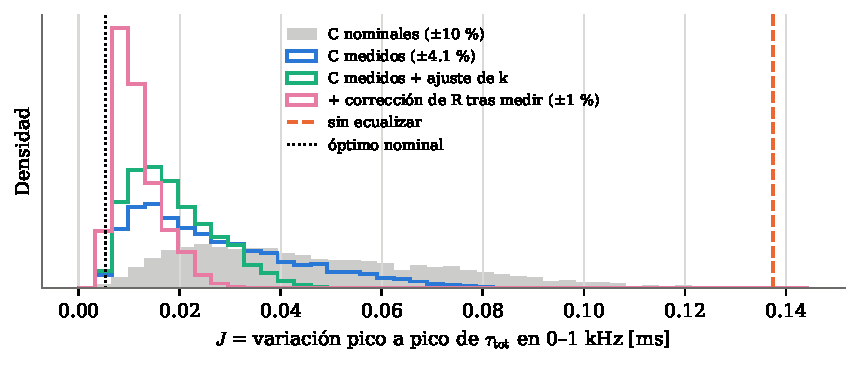
\includegraphics[width=0.8\textwidth]{fig_ec_robustez}
  \caption{Distribución de $J$ para el ecualizador montado sobre el prototipo, según cómo se elijan y ajusten los componentes.}
  \label{fig:ec_robustez}
\end{figure}

\subsection{Simulación}
La \cref{fig:ec_respuesta} muestra la respuesta calculada con los valores de cálculo de la \cref{tab:ec_componentes}. El retardo total queda en unos \qty{0.83}{\milli\second}
y prácticamente constante hasta \qty{1}{\kilo\hertz}; la magnitud del ecualizador es plana, de modo que la de la cascada es la del filtro
desplazada \qty{\eKAPdB}{\decibel}.

\begin{figure}[H]
  \centering
  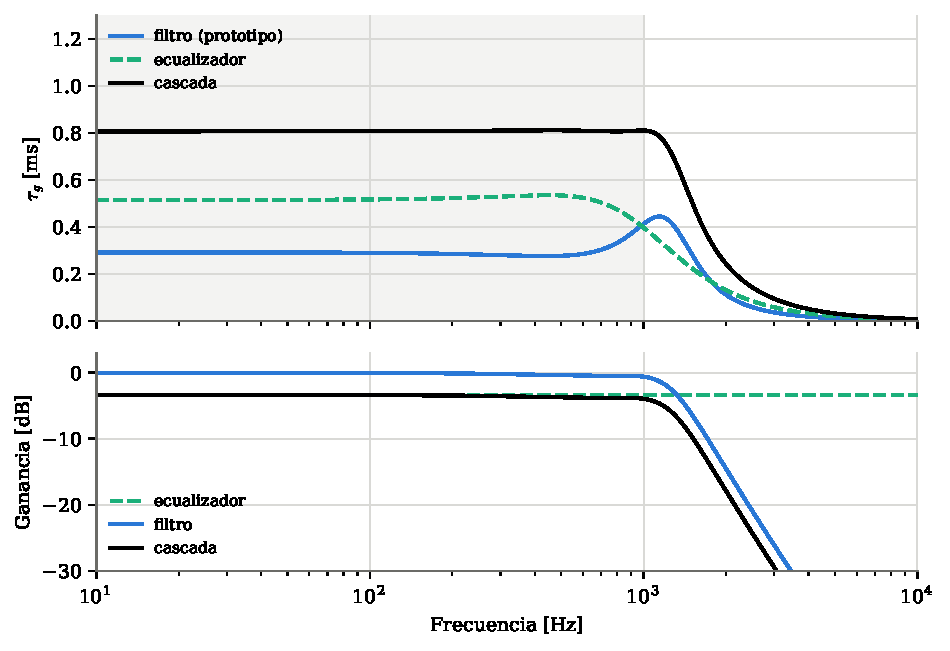
\includegraphics[width=0.85\textwidth]{fig_ec_respuesta}
  \caption{Retardo de grupo y ganancia del filtro (prototipo), del ecualizador y de la cascada, con los valores de cálculo.}
  \label{fig:ec_respuesta}
\end{figure}

Con el modelo, la respuesta al escalón cambia de forma (\cref{fig:ec_escalon_modelo}): el sobrepico baja del \qr{1}{\eSobF}{\percent} al
\qr{1}{\eSobC}{\percent} y aparece una pre-oscilación, del \qr{1}{\ePreC}{\percent}, antes de la subida. La respuesta se vuelve casi simétrica
respecto de su punto medio, que es lo característico de un sistema de fase lineal: la deformación ya no se concentra después del flanco.

\begin{figure}[H]
  \centering
  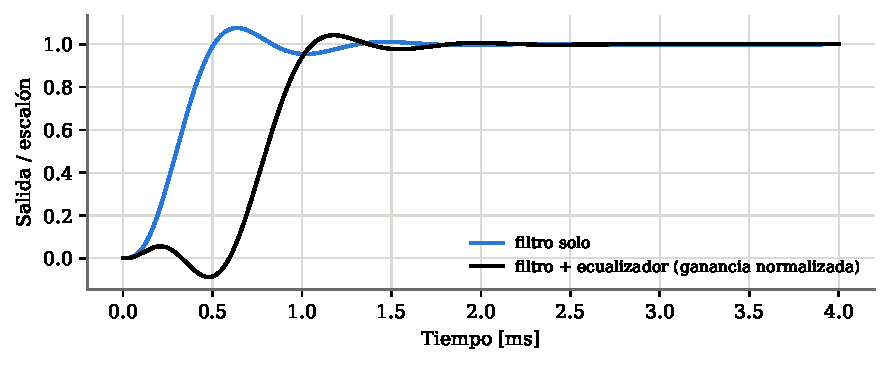
\includegraphics[width=0.8\textwidth]{fig_ec_escalon_modelo}
  \caption{Respuesta al escalón calculada del filtro (prototipo) y de la cascada, normalizada a ganancia unitaria.}
  \label{fig:ec_escalon_modelo}
\end{figure}

En LTspice se simularon el ecualizador solo y la cascada con el ecualizador tal como quedó montado tras la sintonía (resistencias y capacitores
medidos, preset en la posición de magnitud plana), con el macromodelo del TL072 de TI, que comparte etapa de entrada, GBW y slew rate con el TL081
del montaje. La cascada usa el filtro del prototipo reconstruido: resistencias medidas y capacitores estimados en la \cref{sec:mediciones}. Antes, el
netlist del ecualizador se verificó con el solver nodal propio, con un error relativo máximo de \num{\eErrNet} respecto de la transferencia simbólica.
\ifdefined\eLTJCascadaMs
Resultados:
\begin{itemize}
  \item la ganancia del ecualizador es de \qr{2}{\eLTEcGananciaDb}{\decibel} ($20\log k$ con $k = \num{\eKM}$) y varía menos de
        \qr{2}{\eLTEcRizadoDb}{\decibel} entre \qty{10}{\hertz} y \qty{10}{\kilo\hertz}; su retardo difiere del calculado con la transferencia ideal
        en menos de \qr{1}{\eLTEcTauErrMaxUs}{\micro\second} en la banda útil, es decir, el TL081 no introduce error apreciable a estas frecuencias;
  \item la variación del retardo en la banda útil baja de \qr{3}{\eLTJFiltroMs}{\milli\second} (filtro solo) a \qr{4}{\eLTJCascadaMs}{\milli\second}
        (cascada) (\cref{fig:ec_ltspice}). Es una mejora menor que la medida (\cref{sec:ec_medicion}), y la diferencia tiene una causa
        identificable: la simulación usa los capacitores \emph{leídos con el multímetro}, con los que el montaje final da $f_0 = \qr{1}{\eFoM}{\hertz}$
        y $Q = \nr{3}{\eQM}$, un \qty{3.4}{\percent} por encima del objetivo en $Q$. La sintonía, en cambio, se hizo sobre la respuesta medida, es
        decir, sobre los capacitores reales. Los capacitores que explican el $f_0$ y el $Q$ medidos con las resistencias montadas son
        \qty{49.5}{\nano\farad} y \qty{4.63}{\nano\farad}, a $+\qty{4.5}{\percent}$ y $-\qty{3.2}{\percent}$ de las lecturas, del orden de la
        exactitud del UT61D+. La simulación confirma así lo que mostró el análisis de robustez: con capacitores conocidos al
        \qty{4}{\percent}, el ecualizador solo alcanza el óptimo si se sintoniza midiendo;
  \item la respuesta al escalón (\cref{fig:ec_ltspice_escalon}) tiene la forma del modelo: el sobrepico baja del \qr{1}{\eLTEscSobFPct}{\percent} al
        \qr{1}{\eLTEscSobEPct}{\percent} y aparece una pre-oscilación del \qr{1}{\eLTEscPreEPct}{\percent} antes de la subida.
\end{itemize}

\begin{figure}[H]
  \centering
  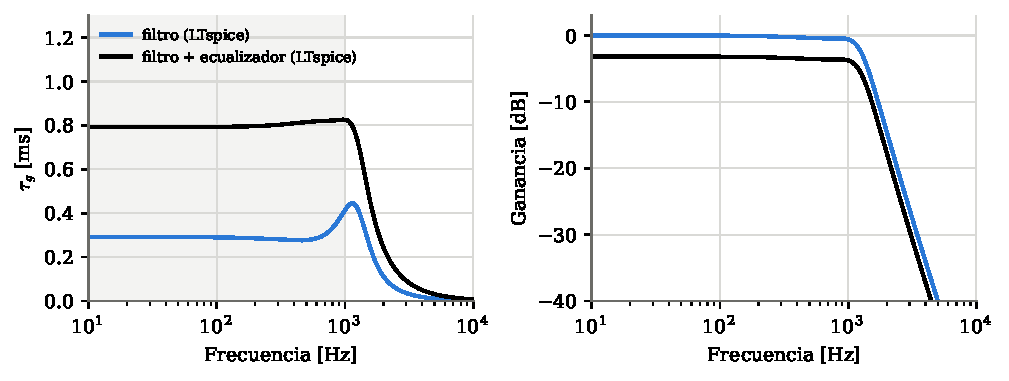
\includegraphics[width=\textwidth]{fig_ec_ltspice}
  \caption{LTspice: retardo de grupo y ganancia del filtro del prototipo solo y con el ecualizador.}
  \label{fig:ec_ltspice}
\end{figure}

\begin{figure}[H]
  \centering
  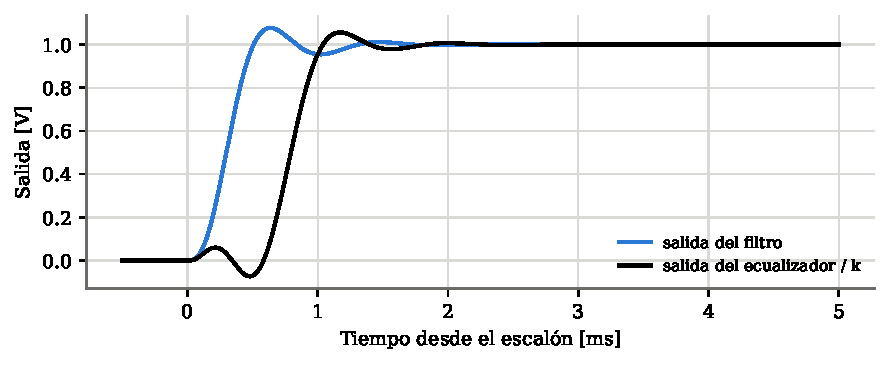
\includegraphics[width=0.8\textwidth]{fig_ec_ltspice_escalon}
  \caption{LTspice: respuesta al escalón de \qty{1}{\volt} a la salida del filtro y a la salida del ecualizador (dividida por $k$).}
  \label{fig:ec_ltspice_escalon}
\end{figure}
\else
\pendiente{correr en LTspice los tres netlists del ecualizador (montaje final) y volver a ejecutar el notebook~06.}
\fi

\subsection{Implementación y medición}
\label{sec:ec_medicion}
El ecualizador se arma con un TL081 a la salida del filtro, con \qty{\pm 12}{\volt} y desacople de \qty{100}{\nano\farad}. El procedimiento
(\texttt{mediciones/nivel3/README.md}) tiene cinco pasos:
\begin{enumerate}
  \item medir los capacitores y las resistencias;
  \item ajustar el preset con el ecualizador solo, hasta que la amplitud de salida a \qty{940}{\hertz} iguale la de \qty{20}{\hertz} (si a
        \qty{940}{\hertz} es menor, $k$ es demasiado grande);
  \item medir con el modo Bode el ecualizador solo y ajustar su modelo ($f_0$, $Q$, $k$, $\varepsilon$) a la ganancia y la fase medidas;
  \item opcionalmente, corregir $R_1$ y $R_2$ si $f_0$ o $Q$ se apartan más de \qty{2}{\percent};
  \item medir la cascada con el modo Bode, con los mismos ajustes que la medición del filtro solo.
\end{enumerate}

Con el Bode del Rigol, el retardo obtenido por diferencias de fase entre puntos vecinos es demasiado ruidoso para resolver variaciones de
\qty{0.01}{\milli\second}. Por eso la mejora se cuantifica de dos maneras independientes: (i) $J$ calculado con el modelo de la cascada ajustado a su
Bode, con su incertidumbre propagada, y (ii) una métrica sin modelo, el desvío de la fase medida respecto de la recta que mejor la aproxima entre
\qty{20}{\hertz} y \qty{1}{\kilo\hertz}. Una fase lineal equivale a un retardo constante, de modo que ese desvío mide directamente la distorsión de
fase. Según el modelo, el desvío máximo pasa de unos \ang{5.6} en el filtro solo a \ang{0.1} con el ecualizador óptimo.

\paragraph{Sintonía.} El ecualizador solo se midió tres veces; entre una medición y la siguiente se cambió la resistencia menor de cada par
(\cref{tab:ec_sintonia}). En cada medición se ajustaron $f_0$, $Q$, $k$ y $\varepsilon$ a la ganancia y la fase, y se calculó el $J$ que daría
el ecualizador sobre el filtro medido.
\begin{itemize}
  \item \textbf{Montaje inicial.} $f_0$ quedó un \qty{4.5}{\percent} por debajo del objetivo. La calibración de canales descartó que el error fuera
        del instrumento. A partir de $f_0$ y $Q$ medidos y de las resistencias montadas se calcularon los capacitores ``efectivos''
        (\qty{48.9}{\nano\farad} y \qty{4.57}{\nano\farad}, a $+\qty{3.3}{\percent}$ y $-\qty{4.4}{\percent}$ de las lecturas, del orden de la
        exactitud del UT61D+) y, con ellos, las resistencias que llevan el
        ecualizador al objetivo.
  \item \textbf{Primera corrección.} Se calculó para el objetivo que daba la estimación preliminar del filtro; por eso, respecto del objetivo final,
        no mejora $f_0$.
  \item \textbf{Segunda corrección (final).} Recalculada con la medición del filtro, deja $f_0$ a un \qty{1}{\percent} del objetivo y $Q$ a menos
        del \qty{0.5}{\percent}. La corrección se eligió con un ajuste preliminar de esa medición (\qty{982}{\hertz} y \num{0.625}); el criterio
        definitivo del notebook~04 da el objetivo de la tabla. Con aquel objetivo, un pasatodo ideal daría $J = \qty{0.0079}{\milli\second}$ en lugar
        de \qr{4}{\eJOpt}{\milli\second}: la diferencia es del orden de la incertidumbre con que se determina $J$ en la cascada
        (\qr{4}{\eMUJCas}{\milli\second}), por lo que no se hizo una tercera corrección.
\end{itemize}
El cambio de resistencias es la forma de sintonizar un circuito cuyos capacitores solo se conocen con la exactitud del multímetro. El preset, en
cambio, solo ajusta la magnitud.

\begin{table}[H]
  \centering\small
  \caption{Sintonía del ecualizador solo: resistencias medidas, $f_0$ y $Q$ ajustados a cada medición, y $J$ previsto sobre el filtro medido. La
  mejora es el cociente entre $J$ del filtro solo (\qr{4}{\eMJFil}{\milli\second}) y $J$ con el ecualizador.}
  \label{tab:ec_sintonia}
  \tabres{tab_ec_sintonia}
\end{table}

\begin{figure}[H]
  \centering
  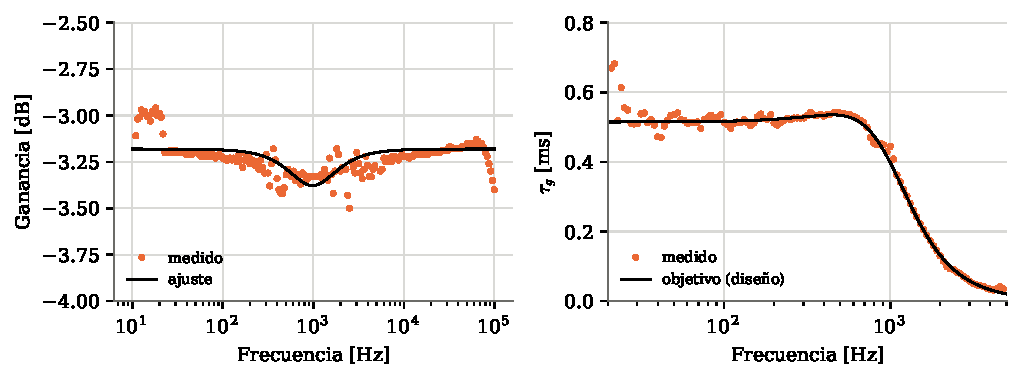
\includegraphics[width=\textwidth]{fig_ec_medicion_ap}
  \caption{Ecualizador solo, montaje final: ganancia y retardo de grupo medidos, con el modelo ajustado y el retardo del ecualizador objetivo.}
  \label{fig:ec_medicion_ap}
\end{figure}

\paragraph{Ecualizador final.} La ganancia es $k = \nr{3}{\eMApK}$ y el error de pasatodo es $\varepsilon = \nr{3}{\eMApEps} \pm \nr{3}{\eMApUEps}$,
es decir, un valle de \qr{2}{\eMApValle}{\decibel} en $f_0$. Su efecto sobre el retardo total está dentro de la incertidumbre: según qué ajuste
se use, el del ecualizador solo o el de la cascada, anularlo con el preset bajaría $J$ o lo dejaría prácticamente igual. Por eso no se retocó el
ajuste. Con ese valle, la atenuación de la cascada en \qty{1}{\kilo\hertz}, referida a su ganancia de continua, sigue por debajo de
\qty{1}{\decibel}.

\paragraph{Cascada.} La \cref{fig:ec_medicion} muestra el retardo de grupo del filtro solo y de la cascada, medidos en la misma sesión. El
retardo del filtro varía entre unos \qty{0.28}{\milli\second} y \qty{0.41}{\milli\second} en la banda de paso; el de la cascada es prácticamente
constante, de unos \qty{0.81}{\milli\second}, hasta \qty{1}{\kilo\hertz}. La consistencia de las mediciones se verificó punto a punto: la fase de la
cascada coincide con la suma de las fases del filtro y del ecualizador medidos por separado, con una diferencia mediana de
\qr{2}{\eMIncMediana}{\degree}. Solo \eMNArtef{} puntos se apartan más de \ang{2}; son errores del instrumento cerca del paso por \ang{-180} y se
excluyen de la métrica sin modelo.

\begin{figure}[H]
  \centering
  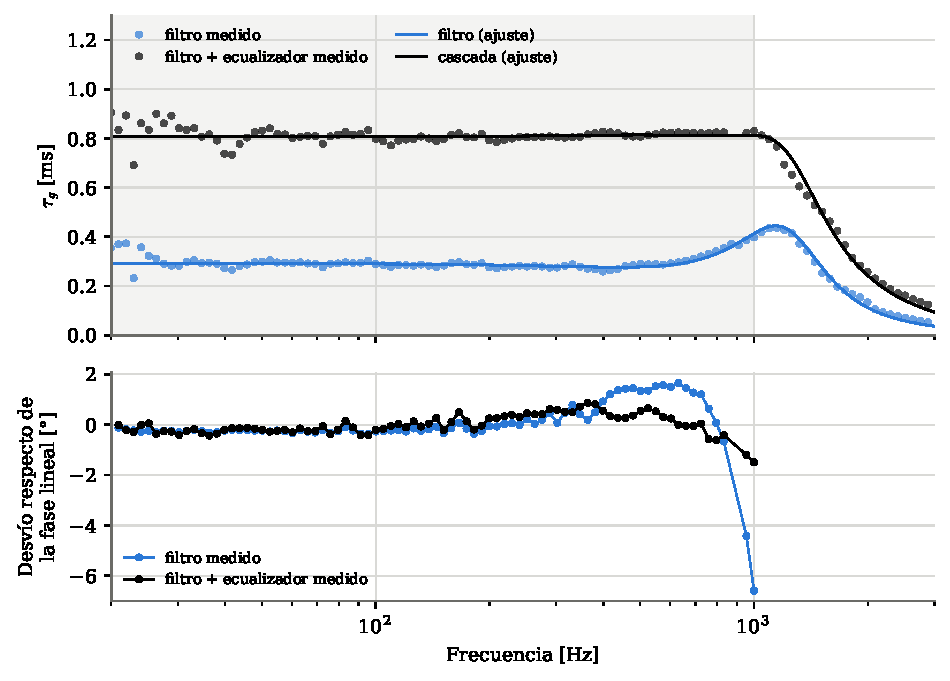
\includegraphics[width=0.95\textwidth]{fig_ec_medicion}
  \caption{Arriba: retardo de grupo medido (regresión local de la fase) del filtro solo y de la cascada, con los modelos ajustados. Abajo: desvío
  de la fase medida respecto de la recta que mejor la aproxima entre \qty{20}{\hertz} y \qty{1}{\kilo\hertz}.}
  \label{fig:ec_medicion}
\end{figure}

\paragraph{Mejora cuantitativa.} Con los dos criterios anunciados:
\begin{itemize}
  \item \textbf{$J$ con el modelo ajustado.} El filtro se ajusta con la medición del filtro solo y, con ese filtro fijo, el ecualizador se ajusta a la
        medición de la cascada. Resulta $J = \qr{4}{\eMJFil}{\milli\second}$ para el filtro solo y $J = \qr{4}{\eMJCas}{\milli\second}$ para la cascada:
        una mejora de \num{\eMMejora} veces, con un intervalo del \qty{90}{\percent} de \numrange{\eMMejoraInf}{\eMMejoraSup} al propagar la incertidumbre
        de ambos ajustes. Calculada con el ecualizador medido por separado, $J$ es de \qr{4}{\eMJPred}{\milli\second} (mejora de \num{10.8}),
        dentro de ese intervalo: $J$ es muy sensible a diferencias de décimas de por ciento en $f_0$, y las dos mediciones las tienen.
  \item \textbf{Sin modelo.} El desvío de la fase respecto de la fase lineal entre \qty{20}{\hertz} y \qty{1}{\kilo\hertz} baja de
        \qr{1}{\eMFilDevMax}{\degree} a \qr{1}{\eMCasDevMax}{\degree} como máximo, y de \qr{2}{\eMFilDevRms}{\degree} a \qr{2}{\eMCasDevRms}{\degree} rms.
        La mejora rms (\num{\eMMejoraFase} veces) es menor que la de $J$ porque el valor de la cascada ya está en el nivel de ruido de fase del
        instrumento, unas décimas de grado.
\end{itemize}
El retardo de la recta pasa de \qr{3}{\eMFilTauLin}{\milli\second} a \qr{3}{\eMCasTauLin}{\milli\second}: es el precio de la ecualización, un
retardo constante adicional de medio milisegundo.

\ifdefined\eEscESobre
\paragraph{Respuesta a la onda cuadrada.} Con una onda cuadrada de \qty{2}{\volt} pico a pico y \qty{50}{\hertz} se registraron a la vez la entrada,
la salida del filtro y la salida del ecualizador (\cref{fig:ec_medicion_escalon}); cada salida se normaliza por su propio escalón. La salida del
filtro tiene un sobrepico de $(\nr{1}{\eEscFSobre} \pm \nr{1}{\eEscFU})\,\%$ y ninguna excursión antes de la subida. A la salida del ecualizador
el sobrepico baja a $(\nr{1}{\eEscESobre} \pm \nr{1}{\eEscEU})\,\%$ y aparece una pre-oscilación de $(\nr{1}{\eEscEPre} \pm \nr{1}{\eEscEU})\,\%$:
el mismo cambio de forma que predice el modelo (\cref{fig:ec_escalon_modelo}), con la deformación repartida a ambos lados del flanco. El cruce
por el \qty{50}{\percent} se demora de \qr{0}{\eEscFTcincuenta}{\micro\second} a \qr{0}{\eEscETcincuenta}{\micro\second}, en acuerdo con el aumento del retardo
de la recta de fase, de \qr{3}{\eMFilTauLin}{\milli\second} a \qr{3}{\eMCasTauLin}{\milli\second}. Las incertidumbres están dominadas por la resolución vertical de la captura, que es
más gruesa a la salida del ecualizador porque su escalón es $k$ veces menor con la misma escala; una captura en modo de alta resolución las
reduciría.

\begin{figure}[H]
  \centering
  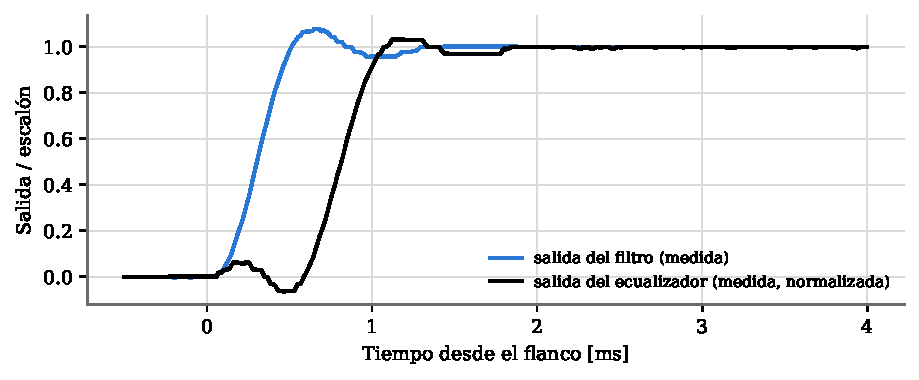
\includegraphics[width=0.9\textwidth]{fig_ec_medicion_escalon}
  \caption{Respuesta medida a una onda cuadrada de \qty{2}{\volt} pico a pico: salida del filtro y salida del ecualizador, cada una normalizada
  por su escalón.}
  \label{fig:ec_medicion_escalon}
\end{figure}
\else
\pendiente{respuesta a la onda cuadrada con el ecualizador final (\texttt{escalon\_cascada.csv}).}
\fi
